\documentclass[letterpaper, 12pt]{report}
\usepackage[spanish]{babel}
\usepackage[latin1]{inputenc}
%\usepackage[T1]{fontenc}
%Options: Sonny, Lenny, Glenn, Conny, Rejne, Bjarne, Bjornstrup
\usepackage[Lenny]{fncychap}
\usepackage{fullpage}
\usepackage{verbatim}
%\usepackage{algorithm}
\usepackage{url}
\usepackage[hidelinks]{hyperref}
%\usepackage{natbib}
\usepackage{graphicx} 
\usepackage{listingsutf8}
\usepackage{color}

\definecolor{mygreen}{rgb}{0,0.6,0}
\definecolor{mygray}{rgb}{0.5,0.5,0.5}
\definecolor{mymauve}{rgb}{0.58,0,0.82}

\lstset{ %
  backgroundcolor=\color{white},   % choose the background color; you must add \usepackage{color} or \usepackage{xcolor}
  basicstyle=\footnotesize,        % the size of the fonts that are used for the code
  breakatwhitespace=false,         % sets if automatic breaks should only happen at whitespace
  breaklines=true,                 % sets automatic line breaking
  captionpos=b,                    % sets the caption-position to bottom
  commentstyle=\color{mygreen},    % comment style
  deletekeywords={...},            % if you want to delete keywords from the given language
  escapeinside={\%*}{*)},          % if you want to add LaTeX within your code
  extendedchars=true,              % lets you use non-ASCII characters; for 8-bits encodings only, does not work with UTF-8
  frame=single,                    % adds a frame around the code
  keepspaces=true,                 % keeps spaces in text, useful for keeping indentation of code (possibly needs columns=flexible)
  keywordstyle=\color{blue},       % keyword style
  language=Octave,                 % the language of the code
  otherkeywords={*,...},            % if you want to add more keywords to the set
  numbers=left,                    % where to put the line-numbers; possible values are (none, left, right)
  numbersep=5pt,                   % how far the line-numbers are from the code
  numberstyle=\tiny\color{mygray}, % the style that is used for the line-numbers
  rulecolor=\color{black},         % if not set, the frame-color may be changed on line-breaks within not-black text (e.g. comments (green here))
  showspaces=false,                % show spaces everywhere adding particular underscores; it overrides 'showstringspaces'
  showstringspaces=false,          % underline spaces within strings only
  showtabs=false,                  % show tabs within strings adding particular underscores
  stepnumber=1,                    % the step between two line-numbers. If it's 1, each line will be numbered
  stringstyle=\color{mymauve},     % string literal style
  tabsize=2,                       % sets default tabsize to 2 spaces
  %title=\lstname                   % show the filename of files included with \lstinputlisting; also try caption instead of title
}

%\bibliographystyle{plain}
\bibliographystyle{ieeetr}
\setcounter{secnumdepth}{3}
\setcounter{tocdepth}{3}
\pagenumbering{roman}

\title{Desarrollo de un Software Libre para la lectura, graficaci�n y registro en tiempo real de se�ales provenientes de ondas cerebrales}
\author{Carlos Antonio Bulnes Dom�nguez}

\begin{document}

\newcounter{rom}


\begin{titlepage}
\maketitle
\end{titlepage}\newpage\thispagestyle{plain}

\addtocounter{rom}{1}\setcounter{page}{2}~
\newpage\thispagestyle{plain}\setcounter{page}{3}

\tableofcontents

\newpage\thispagestyle{plain}~
\clearpage
\pagenumbering{arabic}

\chapter*{Introducci�n}
\markboth{\MakeUppercase{Introducci�n}}{}
\addcontentsline{toc}{chapter}{Introducci�n}

\indent El trabajo presentado describe la realizaci�n de un software libre desarrollado con ROS para ser utilizado con un lector de ondas cerebrales. El nuevo software tiene como objetivo la lectura, graficaci�n y registro de los datos que reciba a trav�s de la plataforma ROS. Durante la investigaci�n se encontr� que ya exist�a un software similar, sin embargo este resultaba muy lento lo que provocaba que la informaci�n en pantalla no fuera fiable. El software resultante en este trabajo tiene como objetivo resolver ese problema, es por eso que, como se explicar� en cap�tulos posteriores, se escogi� integrarlo a ROS.
\\ \indent El nuevo software permitir� controlar el momento en que se quiera Ejecutar, Pausar y Detener la recepci�n de la informaci�n, estas acciones no afectar�n al programa que env�a los datos pues solo afecta de forma visual al programa receptor para que el usuario tenga control de que quiere ver y en que momentos. Adicionalmente cuenta con la funcionalidad de visualizar y crear un registro de todas las se�ales que se reciban mientras el software se encuentre en modo de ``reproducci�n''. La visualizaci�n es e tiempo real mientras que la generaci�n del registro se genera cuando se presiona ``detener'' y crear� un archivo en disco duro con el nombre que se haya ingresado as� como la fecha y hora de creaci�n de este, dicho archivo permitir� al usuario consultarlo en cualquier momento independientemente de que el software se encuentre en ejecuci�n o no.\newpage\cleardoublepage
\chapter*{Justificaci�n}
\markboth{\MakeUppercase{Justificaci�n}}{}
\addcontentsline{toc}{chapter}{Justificaci�n}


La necesidad de la creaci�n de un software libre para la lectura de las ondas cerebrales surge debido a la escaza variedad de programas dedicados a dicha tarea actualmente, donde es el mismo creador del dispositivo f�sico el que te proporciona el software, el cual, ya cuenta con funciones y operaciones definidas por el fabricante.
\\ \indent
En la actualidad los proyectos de investigaci�n requieren interactuar m�s con la informaci�n que obtienen con los dispositivos lectores de ondas cerebrales, y como ya se mencion�, las alternativas actuales se encuentran limitadas, se propone entonces un proyecto de c�digo libre en el cual, partiendo del software desarrollado en este trabajo, los desarrolladores futuros sean capaces de complementarlo e implementarlos a sus necesidades espec�ficas.
\newpage\cleardoublepage
%\section*{Hip�tesis}
\markboth{\MakeUppercase{Hip�tesis}}{}
\addcontentsline{toc}{section}{Hip�tesis}
El software desarrollado leer� las se�ales de un EEG y las graficar�. Las gr�ficas ser�n en tiempo real, las cuales estar�n monitoreando las se�ales recibidas en una relaci�n frecuencia-tiempo (como lo hace un Osciloscopio electr�nico). Adem�s se podr�n obtener dichos datos en valores num�ricos para que as� el software pueda comunicarse con otras herramientas.
\newpage\cleardoublepage
\section*{Objetivos}
\markboth{\MakeUppercase{Objetivos}}{}
\addcontentsline{toc}{section}{Objetivos}

\subsection*{Objetivo General}
\markboth{\MakeUppercase{Objetivo General}}{}
\addcontentsline{toc}{subsection}{Objetivo General}
%Crear un software libre capaz de interpretar las se�ales de un EEG para que puedan ser usadas por medio de herramientas externas.
Crear un software libre capaz de leer y graficar en tiempo real a trav�s de la plataforma ROS las se�ales enviadas por el Emotiv EPOC, las cuales son interpretadas por un software libre llamado emokit\cite{emokit}.

\subsection*{Objetivos Particulares}
\markboth{\MakeUppercase{Objetivos Particulares}}{}
\addcontentsline{toc}{subsection}{Objetivos Particulares}

\begin{itemize}
\item Establecer un canal de comunicaci�n entre el software y el EEG.
\item Obtener datos num�ricos a partir de las se�ales obtenidas.
\item Tomar esos datos en tiempo real y graficarlos en una relaci�n frecuencia-tiempo.
\item Establecer un canal de salida para enviar los datos interpretados.
\end{itemize}\newpage\cleardoublepage
\section*{Antecedentes}
\markboth{\MakeUppercase{Antecedentes}}{}
\addcontentsline{toc}{section}{Antecedentes}

El software desarrollado en este trabajo toma como base al emokit\cite{emokit} el cu�l forma parte de OpenYou\cite{emokit}. El Emokit lee, descifra e interpreta la informaci�n enviada por el Emotiv EPOC, el cual es un dispositivo ``Interfaz Cerebro-M�quina'' (BCI), tales como nivel de bater�a de la diadema, intensidad de la se�al, y las 14 lecturas realizadas por la diadema; este software actualmente solo imprime a nivel terminal dichos datos.
\\ Una ``Interfaz Cerebro-M�quina''\cite{2012bci} (BCI) es un medio de comunicaci�n directo entre el cerebro y un dispositivo externo. Los BCI est�n normalmente dirigidos a asistir, aumentar y reparar la habilidad cognitiva y las funciones sensoriomotoras.
\\ Las inventigaciones con los BCI comenzaron en 1970 en la Universidad de Los �ngeles California(UCLA) bajo el subsidio de Fundaci�n Nacional de Ciencia contratados por la Agencia de Proyectos de Investigaci�n Avanzados de Defensa (DARPA). La publicaci�n hecha despu�s de la investigaci�n marc� la primera aparici�n de la expresi�n ``Interfaz Cerebro-M�quina'' en la literatura cient�fica. En la actualidad existen tres tipos de BCI:
\begin{itemize}
\item BCI invasivos: Son implantados en la materia gris del cerebro por medio de una neurocirug�a, debido a que se encuentran implantados en el cerebro los BCI invasivos producen la mejor calidad de las se�ales pero pueden tener consecuencias negativas al portador a futuro.
\begin{figure}[htb]
\centering
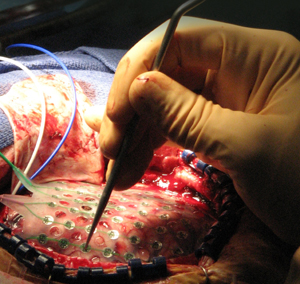
\includegraphics[width=0.4\textwidth]{img/bci1.jpg}
%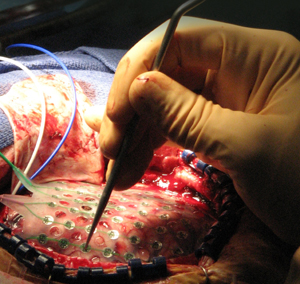
\includegraphics[scale=1,bb=0 0 30 30]{img/bci1.jpg}
\caption{BCI invasivo\cite{img:invasive-bci}} \label{fig:bci1}
\end{figure}

\item BCI semi invasivos: Son implantados dentro del cr�neo pero sin tocar la corteza cerebral. Producen una mejor se�al que los BCI no invasivos y tienen menor riesgo de causar da�os al cerebo que los BCI invasivos.

\item BCI no invasivos: Los implantes no invasivos son colocados en el cuero cabelludo. Los BCI no invasivos producen se�ales d�biles porque el cr�neo amortigua las se�ales, dispersando las ondas electromagn�ticas creadas por las neuronas.
\begin{figure}[htb]
\centering
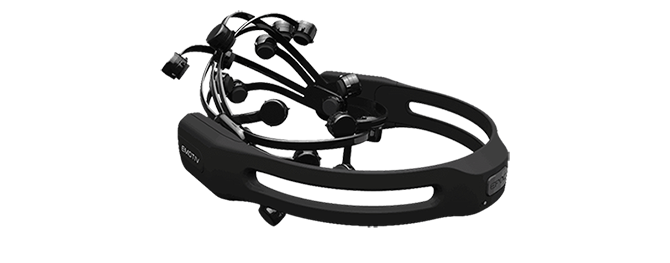
\includegraphics[width=0.8\textwidth]{img/epoc.png}
%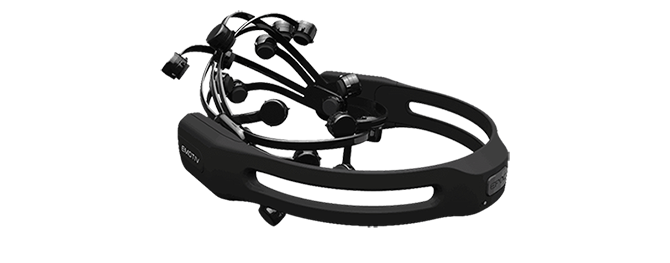
\includegraphics[scale=1,bb=0 0 30 30]{img/epoc.png}
\caption{BCI no invasivo\cite{emotiv:Online}} \label{fig:bci2}
\end{figure}

\end{itemize}

\subsection*{BCI Invasivos}
\markboth{\MakeUppercase{BCI Invasivos}}{}
\addcontentsline{toc}{subsection}{BCI Invasivos}

Los dispositivos BCI invasivos son implantados directamente en el cerebro y tienen la m�s alta calidad de se�ales de los BCI. Estos dispositivos son usados para recuperar funciones de personas con par�lisis. Los BCI invasivos son usados tambi�n para recuperar la vista conectando el cerebro a c�maras externas y para restaurar el uso de extremidades usando brazos y piernas rob�ticos controlados por el cerebro. Como todos los dispositivos que se encuentran instalados en la materia gris del cerebro este tipo de BI produce una calidad de se�ales muy alta pero son propensos a causar cicatrices en el tejido cerebral causando que las se�ales comiencen a volverse d�biles o incluso la p�rdida de las reacciones del cuerpo por contener un objeto desconocido en el cerebro\cite{invasiveBCI1}. \\
En las ciencias de la visi�n los implantes en el cerebro han sido usados para tratar la ceguera no cong�nita\footnote{Una enfermedad cong�nita es aquella que se manifiesta desde el nacimiento, ya sea por un trastorno ocurrido durante el desarrollo embrionario, durante el parto o como consecuencia de un defecto hereditario}. William Dobell es uno de los primeros cient�ficos que vienen trabajando con una interfaz cerebro para restaurar la vista como una investigaci�n privada. El implant� su primer prototipo en Jerry, un hombre que qued� ciego en su adultez en 1978. �l insert� un BCI de 68 electrodos en la corteza visual de Jerry y logr� producir la sensaci�n  de ver una luz. En 2012 el experimento fu� realizado en Jens Neumann donde Dobell utiliz� un implante m�s sofisticado que permiti� un mejor mapeo. Investigadores de la Universidad de Emory en Atlanta, dirigidos por Philip Kennedy y Roy Bakay fueron los primeros en instalar un implante en el cerebro de un ser humano que produce se�ales de alta calidad suficientes para estimular el movimiento\cite{invasiveBCI1}. \\
Thomas Navin Lal et al. en su art�culo \cite{invasiveBCI1} desarrollaron un BCI llamado Thought Translation Device (TTD) es cual usan para ayudar a comunicarse a pacientes con par�lisis los cu�les han perdido sus funciones cognitivas. Para poder usar el TTD los pacientes debieron aprender a regular a voluntad su Slow Cortical Potentials (SCP)\footnote{Se llaman SCP (o potenciales corticales lentos en espa�ol) a los cambios relacionados con los eventos de corriente continua lenta obtenidas con los EEG provenientes de los grandes conjuntos de c�lulas en la capa cortical superior\cite{SCP:Online}.}. El sistema entonces permite a su usuario escribir textos en la pantalla de una computadora o navegar en internet. El sistema sin embargo cuenta con dos desventajas: no todos los pacientes logran controlar su SCP adem�s la intensidad de la se�al es un poco baja y a un usuario bien entrenado requiere aproximadamente 30 segundos para escribir un caracter. % insertar imagen del articulo
\newpage\cleardoublepage



El Emotiv Epoc es BCI que fue creado con el prop�sito de ser un perif�rico para juegos en Windows, OS X y Linux\cite{Emotiv:Wiki:Online}, cuenta con 14 electrodos y funciona como dispositivo de entrada. En 2011 Kirill Stytsenko, et al.\cite{stytsenko2011evaluation} realizaron un an�lisis del Emotiv EPOC para la CogSci Conference. Emotiv EPOC es un BCI de bajo costo basado en la tecnolog�a EEG. Cuenta con 14 electrodos montados en una diadema inal�mbrica que se coloca sin esfuerzo y se conecta a la computadora. Originalmente fue creada para los juegos de computadora pero la ``research edition'' permite el acceso a los datos para su an�lisis lo que abre nuevas posibilidades a la ciencia para realizar nuevos experimentos o integrarlo a los ya existentes. En dicho estudio se someten a diferentes pruebas al Emotiv EPOC y al G-TEC\cite{G-TEC:Online}. Al compararlos se obtiene que la informaci�n en general es igual, pero la se�al es m�s clara e intensa en el G-TEC. Uno de los desaf�os encontrados es la creaci�n de software de grabaci�n para ambos dispositivos.
\\ Job Ram�n de la O Ch�vez en su tesis Interfaz Cerebro - Computadora para el Control de un Cursor Basado en Ondas\cite{intcerebro} plantea una interfaz que permita la comunicaci�n entre el usuario y la computadora, haciendo uso de sus ondas cerebrales, para el control de un cursor en pantalla mediante comandos obtenidos de las lecturas de un amplificador de ondas cerebrales.
\\ En EPOC-alypse Mind Controlled Car\cite{seniorepoc} plantean la construcci�n de de un carro de control remoto que es controlado por la mente usando el Emotiv EPOC. El proyecto fue desarrollado utilizando el SDK oficial del Emotiv EPOC.
\\ Asim Raza en SSVEP based EEG Interface for Google Street View Navigation\cite{raza2012ssvep} analiza los sistemas BCI y su aplicaci�n en el mundo real. Tambi�n desarrolla un prototipo interactivo que pueda ser controlado en un ambiente controlado para demostrar el funcionamiento de los sistemas BCI. Para el desarrollo decidi� utilizar el software libre OpenViBE para la adquisici�n y procesamiento de las se�ales.
\\ En ROS: an open-source Robot Operating System\cite{2009ros} se explica el uso de la plataforma ROS para el desarrollo de aplicaciones de rob�tica y resumen los objetivos filos�ficos de ROS en:
\begin{itemize}
\item Per-to-per
\item Basado en herramientas
\item Multilenguaje
\item Ligero
\item Gratuito y de C�digo Abierto
\end{itemize}
%ROS provee una capa de comunicaci�n estructura basada en Peer-to-peer, basado en herramientas, adem�s es multilenguaje, ligero, gratuito y de c�digo abierto.
En Things that twitter: social networks and the internet of things\cite{kranz2010things} utilizan ROS aplicado en las redes sociales. ROS permite intercambiar informaci�n por medio de servicios con mensaje de request y response definidos. La informaci�n es intercambiada por una arquitectura publish/suscribe donde los procesos permiten que sus datos est�n disponibles para que otros procesos puedan utilizarlos.

% Trabajos sobre cda tipo de BCI, enfatizar no invasivo.
% LIrbos, publicaciones etc que hablen sobre ellos.
% aplicacion en los videojuegos
% Avance de las compa�ias en el tema de los BCI
% Quienes han investigado sobre BCI
% Paises avanzados en el campo
% Campos con los que se relaciona\newpage\cleardoublepage
\chapter*{Dise�o}
\markboth{\MakeUppercase{Dise�o}}{}
\addcontentsline{toc}{chapter}{Dise�o}

\indent La Universidad Veracruzana adquri� un Emotiv EPOC en 2014 para el laboratorio de rob�tica donde los alumnos de la Facultad de Ingenier�a participan en diferentes proyectos tecnol�gicos. Este trabajo de tesis contribuye a un proyecto donde se controlar� un robot por medio de la mente a trav�s del Emotiv EPOC. Con el proyecto resultante de este trabajo se tendr� una interfaz la cual graficar� las se�ales del Emotiv EPOC adem�s de tener la capacidad de grabar los datos obtenidos cada vez que se ejecute un ``experimento'' obteniendo un archivo separado por comas.
\\ \indent Al momento de la investigaci�n se encontraron algunos software que mostraban la informaci�n obtenida de forma gr�fica, sin embargo el principal inconveniente de estos era el desfase entre los datos que se estaban obteniendo y su graficaci�n. Para atacar ese problema en este proyecto se utiliz� un framework llamado ROS. ROS (Robot Operating System)\cite{ROS:Wiki:Online} provee librer�as y herramientas para ayudar a los desarrolladores de software a crear aplicaciones para robots. ROS provee abstracci�n de hardware, controladores de dispositivos, librer�as, herramientas de visualizaci�n, comunicaci�n por mensajes, administraci�n de paquetes y m�s. ROS est� bajo la licencia open source, BSD. En este proyecto se utiliz� ROS para crear un escenario de comunicaci�n en tiempo real, donde el Emokit\cite{emokit} publica a trav�s de mensajes los datos obtenidos del Epoc as� mismo el nuevo software leer� los mensajes publicados en ROS para obtener los datos para graficarlos y generar el ``log'', todo esto ya en tiempo real.
\\ \indent Para la construcci�n del software presentado en este trabajo se utiliz�:
\begin{itemize}
\item Python\footnote{ Lenguaje de programaci�n que puede ser usado para diferentes prop�sitos como aplicaciones web, aplicaciones de escritorio, int�rprete, etc}
\item PyQT\footnote{  Binding de la biblioteca gr�fica Qt para el lenguaje de programaci�n Python}
\item Matplotlib\footnote{ Biblioteca para la generaci�n de gr�ficos a partir de datos contenidos en listas o arrays en el lenguaje de programaci�n Python y su extensi�n matem�tica NumPy}
\item ROS
\end{itemize}
\newpage\cleardoublepage
\chapter*{Implementaci�n y Resultados}
\markboth{\MakeUppercase{Implementaci�n y Resultados}}{}
\addcontentsline{toc}{chapter}{Implementaci�n y Resultados}

La impelmentacion es una explicacion del software funcionado e imagenes de esllo
%Capturas y fotos de la aplicacion funcionando e interactuando con la diadema
\\ \indent A continuaci�n se presentan los c�digos con los que fue posible este proyecto, el proyecto completo puede ser descargado en \url{http://github.com/carlosbulnes/epoc/}.

Primero tenemos al c�digo del emokit adaptado a ROS.
%\lstinputlisting[language=Python, caption=emokit.py]{code/emokit.py}

El c�digo del software realizado en este trabajo es el siguiente. Este est� constituido por un programa principal llamado interfaz.py el cu�l depende de los c�digos GUI.py que es la definici�n de la interfaz en PyQT y matplotlibwidgetFile.py que permite la integraci�n de matplotlib a PyQt.
\\ 
%\lstinputlisting[language=Python, caption=interfaz.py]{code/interfaz.py}
%\lstinputlisting[language=Python, caption=GUI.py]{code/GUI.py}
%\lstinputlisting[language=Python, caption=matplotlibwidgetFile.py]{code/matplotlibwidgetFile.py}
%C�digos y su desarrollo
%Versiones
\newpage\cleardoublepage
\chapter*{Conclusi�n y trabajo futuro}
\markboth{\MakeUppercase{Conclusi�n y trabajo futuro}}{}
\addcontentsline{toc}{chapter}{Conclusi�n y trabajo futuro}

Se logr� crear un software el cual es capaz de leer mensaje publicados en ROS para generar las graficas y el registro. La principal ventaja es que al ser en ROS su funcionamiento en base a mensajes esto permite que sea usado en cualquier escenario que publique el mismo tipo de mensaje que el software lee y no se encuentra limitado a funcionar unicamente con el emokit o incluso para el Emotiv Epoc.

\section*{Trabajo Futuro}
\markboth{\MakeUppercase{Trabajo Futuro}}{}
\addcontentsline{toc}{section}{Trabajo Futuro}

Al ser libre, es software en este poryecto puede ser mejorado de muchas formas y para distintos prop�sitos. \newpage\cleardoublepage

%\listofalgorithms
\listoffigures
%\listoftables

\markboth{\MakeUppercase{Bibliograf�a}}{}
\addcontentsline{toc}{chapter}{Bibliograf�a}
\bibliography{bib/Bibliografia}\newpage\cleardoublepage

\end{document}